The \ivfprototype{} was evaluated based on the implemented functions.
These functions are structured to the research workflow as described in figure \ref{fig:functions-workflow}. 
This workflow will now be referred to as the `process' of the system.

For the purpose of the evaluation the \ivfprototype{} code was running on the local environment of a laptop.
No connection to the internet was necessary for testing, therefore performance issues were out of the question.
The used dataset was randomly generated (strings of letters), because the \projectdata{} was not available yet.
Screenshots of the running gateway are shown in figures \ref{fig:standard-view-website} and \ref{fig:sunburst-view-zoom-website}.

\begin{figure}[!b]
	\centering
	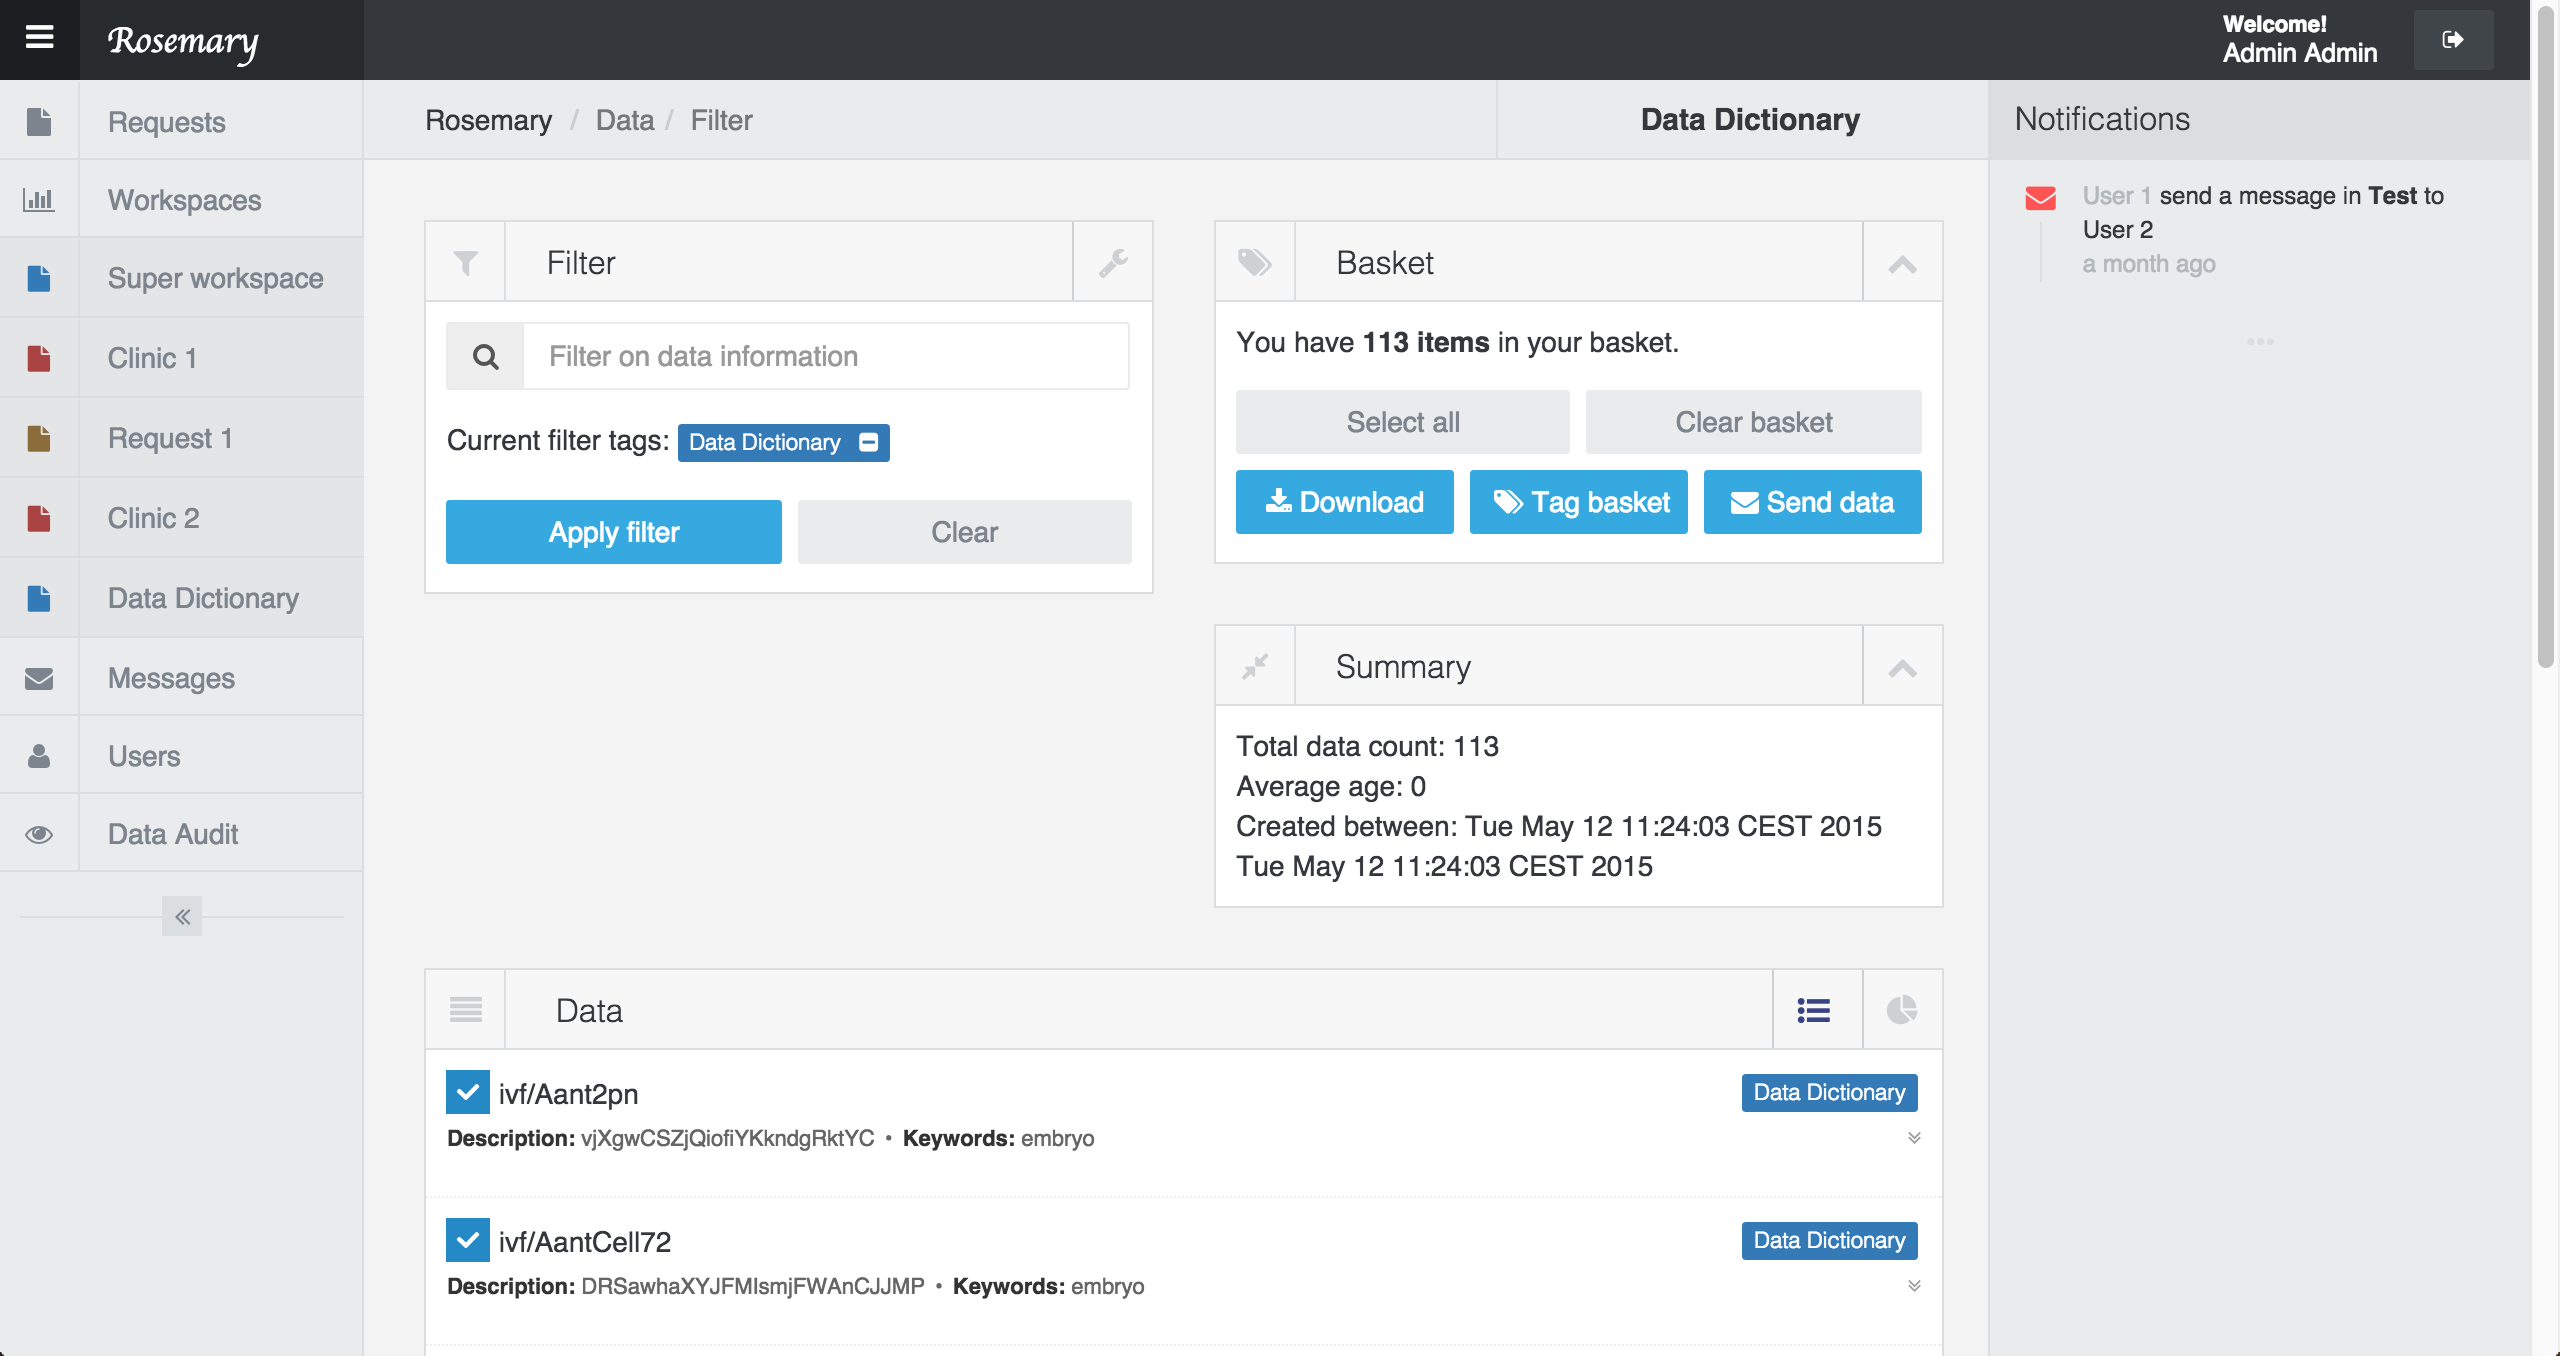
\includegraphics[width=1.0\linewidth]{images/standard-view}
	\caption{
		Running \ivfsystem{} data management view showing the standard display of the data (\ie{} summary on top and raw data at the bottom).
	}
	\label{fig:standard-view-website}
\end{figure}

\begin{figure}[ht]
	\centering
	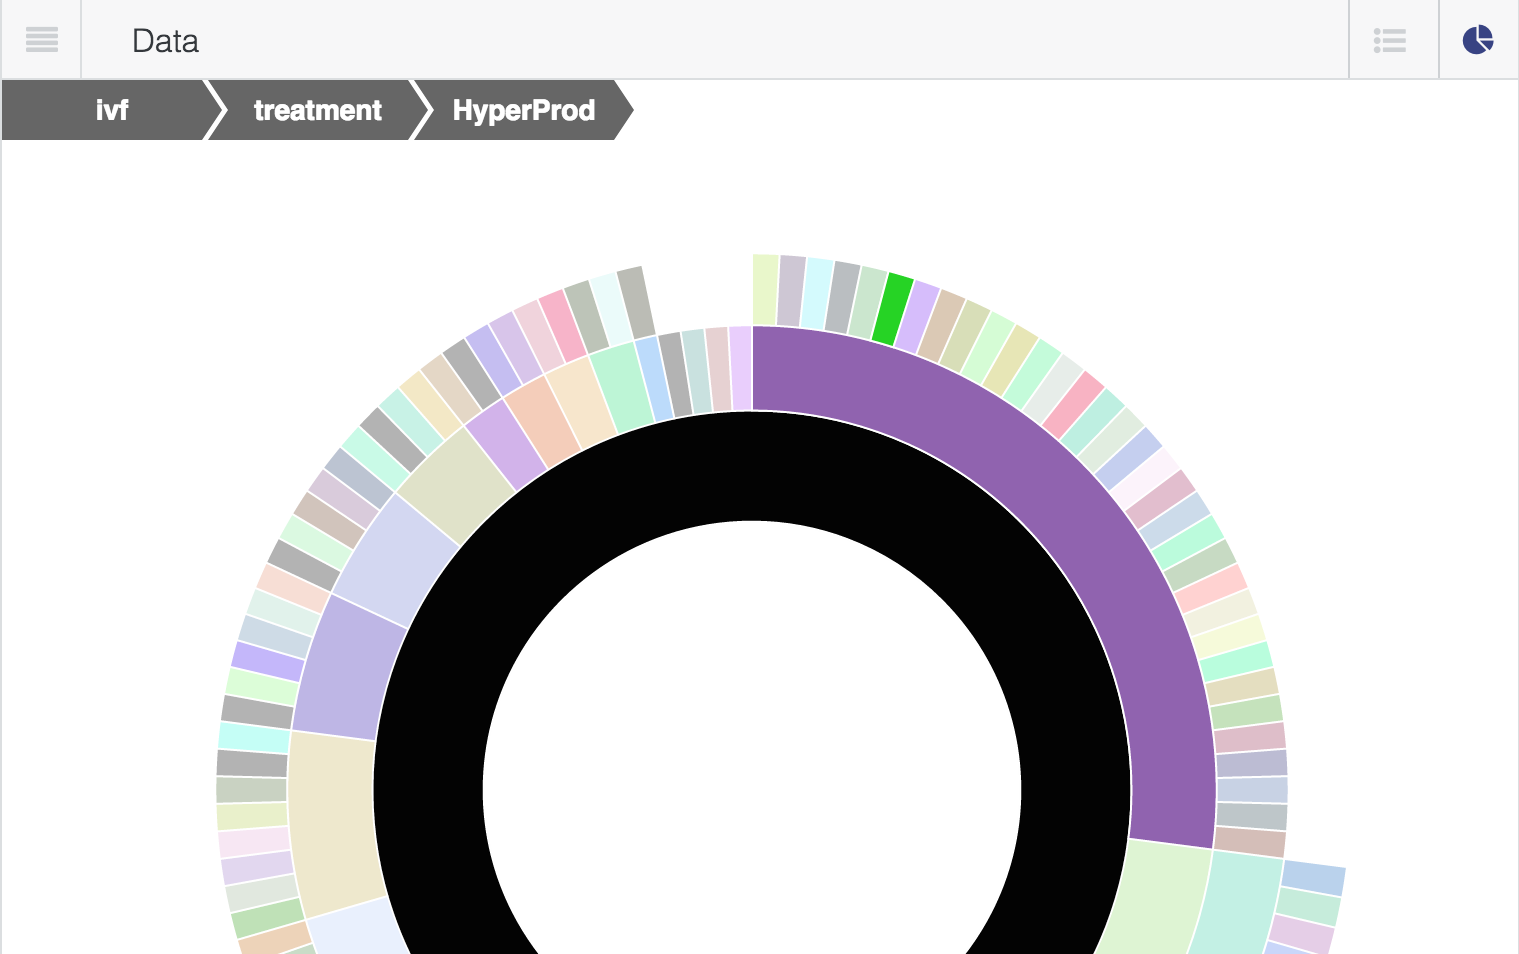
\includegraphics[width=0.7\linewidth]{images/sunburst-closeup}
	\caption{
		Running \ivfsystem{} data graph view showing the (sunburst) graph display of the data.
	}
	\label{fig:sunburst-view-zoom-website}
\end{figure}

All evaluations were done in an informal open-talk setting with no predefined questions, the testers were encouraged to think aloud.
First, the purpose of the meeting was explained in a few sentences.
Each user had to perform tasks using the prototype according to the assigned case: researcher, committee, administrator.
There were three testers, and some were assigned two cases because they fit in the field of experience of the respective user role.

Tasks were described according to the system schema presented in figure \ref{fig:brainstorm-after}.
No explanation was given about the user interface and the concepts (\eg{} filter or basket components), these had to be discovered by the tester.
The interviewer only gave directions during the evaluation after the tester indicated that they did not know how to proceed.
If a bottleneck was encountered testers were asked to suggest design or process alternatives.

The  cases presented below are loose transcripts of the evaluation sessions.
The transcripts will be structured like: task description, how the task should be performed, how the tester performed the task, and comments and difficulties.
After these the results are summarised in section \ref{evaluation-summary}.
First the design will be summarised using Nielsen's ten heuristics \cite{designHeuristics} and then general notes about the system are described.

\section{User sessions transcripts}

\paragraph{Researcher Role}
From all the cases this is arguably the largest as it has the most extensive (implemented) functions.
The tasks that had to be performed were: search the data dictionary for headers, use these data headers to compose and submit a request, download the requested data.

Testers had to find the data dictionary and use the filter function to search for the headers they wanted to use.
They could also use the graph shown in figure \ref{fig:sunburst-view-zoom-website} to find what they were looking for.
After finding the wanted headers they are added to the basket by selecting them - when using the data dictionary the basket is used for `shopping' data where the request is the `checkout' and submitting the request places the `order'.

After the basket is filled with the wanted data the user navigates to the `new request' form.
In this form the headers from the basket are automatically added and the user fills out the other required information (\eg{} research question, description).
When the request is submitted the user waits for approval; for the evaluation an approved request was provided for the download task.

Downloading data is achieved by navigating to the wanted workspace in the menu on the left side of the screen.
Users can either make a small selection or click the `select all' button to add data to their basket.
By clicking the `download' button in the basket the system provides a downloadable file.

Finding the data dictionary was no problem for the testers.
The next step is filtering, which is relatively easy as the input is text based and the search itself is fuzzy.
More extensive functions of the filter are not directly apparent but after a short explanation users could apply them to search for items based on name, description, and keywords.

Two of the testers did not notice that the search is instantaneous (like google search).
This resulted in pressing 'enter' and clicking the `apply filter' button multiple times before noticing that the data had already changed at the bottom of the screen.
One of the testers prefers to search the data off-line, \ie{} print the fields and later select the wanted items in the interface.

Because in the prototype the descriptions are nonsense, it was difficult to find the wanted data headers.
Therefore, testers were asked to select a couple of random headers.
Selection was straightforward but the testers did not notice that selected items were added to the basket.
Therefore, two asked `how do I keep this selection when I start searching again?'.
This also resulted in two of the testers using the `select all' function on the basket.
Clicking this will make a selection of \emph{all} the items in the workspace, basically overwriting the previous basket and losing all the progress.

To proceed in the task of making a request the testers looked for a button on the basket.
However, the buttons are specific to a 'data view' and do not make sense in a 'dictionary view' of the system.
The testers needed to be explained that the basket is kept in the back of the system and can be used over multiple views.
After this comment the tester could quickly find the `new request' form fill it out and submit it.

Data download is straightforward. 
No problems were found here, one of the testers noted that in principle \emph{all} data will be downloaded every time.
In this case the `select all' button on the basket helped them.

\paragraph{Committee Member Role}
The committee tasks are the shortest, as the list only contains the request approval function. 
It breaks down into finding the requests which are open for approval, evaluating them against already approved requests, optionally communicating with other committee members, and voting.
Viewing requests that are ready for approval is done by selecting the `request' button from the left menu.
Now a list is shown of all these requests and the data that is necessary for making the decision.
Clicking on one of the requests redirects to `new message', the user can create a message which (upon clicking send) is automatically send to all committee members.
Approval is given (or not) by selecting a approve or disprove button, a vote remains open for change until all committee members have casted their vote.
The actual vote is shown both with a symbol (\checkmark{}/\texttimes{}) as with a colour (green/red).

Generally the process was clear to the tester, finding the proper request and voting went smoothly.
The tester tried to click on a request to view more information, even though all the available information was already shown.
The click leads to the `new message' which confused the tester.
There was a suggestion to add a comments thread to the request itself, instead of the separate message construction.
And even though they did not explicitly say it, it can be discerned that the tester needed more information on the request.

One tester (an P.I.) mentioned that the request management functions might help them when doing grant applications.
Saying that many funding sources require that after the funded research is completed that data is available for reuse.
Demoing the system and adding it to the grant application might give them a better position for getting the fund.
What was also mentioned is that giving data deliverers (\ie{} key persons from each clinic) the possibility to keep a certain `hold' over their own data might increase their willingness to provide their data.

\paragraph{Data administrator Role}
Lastly, the data administrator performed the user management functions.
This is done by finding the needed user in a list and changing the wanted setting (\ie{} is committee member, is active, is approved).
After selecting the `users' button from the left menu the list of users is shown. 
Each user contains buttons to change each of the settings, \ie{} make (or unmake) committee member, make (in)active, and (un)approve.
The status for each of these settings is given with a symbol (\checkmark{}/\texttimes{}) and with a colour (green/red).

User management was clear and would be easy to use in a real-life scenario.
However, the tester noticed that a system requirement was not discovered yet.
If one of the users of the system changes institutions, most of the time the data manager is not informed, this is left to the P.I.s (which are not included in the \ivfsystem{} requirements).
This is important when, for example, a committee user starts working for a different clinic thereby losing the role of committee member.
Or when a researcher changes institutions and access to a previous data request should be revoked.
Therefore the system should contain functions for non-administrators to view the list of users and communicating with the data manager about what actions should be taken.